\section{WKB Approximation}
The WKB approximation is a semiclassical approximation 
for an eigenstate when the rate of change of the potential 
is much smaller than the oscillation frequency (momentum) of the eigenstate. 
Consider the one-dimensional Schrodinger equation again 
\[ 
    -\df {\hb^2}{2m}\pd {x}^2 \psi(x) + V(x)\psi(x) = E\psi(x)
\] 
Let $p(x)\equiv \sqrt{2m[E-V(x)]}$, this may be rewritten as 
\begin{equation}\label{eqn:1d schrodinger in momentum}
    \pd x^2\psi = -\df{p^2}{\hb^2}\psi
\end{equation}
Substitute the following solution expression, for $A$ and $\phi$ real functions:
\[
    \psi(x) = A(x) \exp[i\phi(x)]
\] 
Calculate the first and second order derivatives 
\malign{
    \pd x \psi &= (A'+i\phi')\exp(i\phi) \\ 
    \pd x^2 \psi &= \left[A'' + 2iA'\phi' + iA\phi'' - A(\phi')^2\right]\exp(i\phi)
}
Substitute into the Schrodinger equation~\ref{eqn:1d schrodinger in momentum}, 
we have 
\[ 
    A'' + 2iA'\phi' + ia\phi'' - A(\phi')^2 = -\df{p^2}{\hb^2}A
\] 
Separate into real and imaginary components:
\begin{equation}\begin{aligned}\label{eqn:se_wkb}
    A'' - A(\phi')^2 = -\df{p^2}{\hb^2} A &\iff A'' = A\left[(\phi')^2 - \df{p^2}{\hb^2}\right]  \\ 
    2A'(x)\phi'(x) + A(x)\phi''(x) = 0 &\iff \pd x \left(A^2(x)\phi'(x)\right) = 0
\end{aligned}\end{equation}
The second equation implies that $A^2(x)$ is constant, let $\alpha = A^2(x)\phi'(x)\in \R$. Then 
\[ 
    A(x) = \df{\alpha}{\sqrt{\phi'(x)}}
\] 
We're left with solving the real equation with only $\phi$. 
Note that when $V(x)$ is constant, we have the free-particle solution 
\[ 
    \psi(x) = A\exp\left(\df i \hb p x\right), \quad \phi(x) = \df 1 \hb p x
\] 
WKB makes the following power series expansion of $\phi(x)$ ($S_0$ has units of action). 
The variable is in $\hb^2$ due to $\hb^2/2m$ term in Schrodinger equation. 
\[ 
    \phi(x) = \df 1 \hb \sum_{n=0}^\infty \hb^{2n}S_n(x) = \df 1 \hb S_0(x) 
    + \hb S_1(x) + \hb^3 S_2(x)+\cdots
\] 
Substitute this into the first equation in~\ref{eqn:se_wkb} and equate by powers of $\hbar$. 
Taking the first term 
\[\begin{aligned} 
    \phi'(x) &= \df 1 \hb S_0'(x) + \hb S'_1(x) \\ 
    A(x) &= \df {\alpha}{\sqrt{\frac 1 \hb S'_0(x) + \hb S'_1(x)}}
\end{aligned}\] 
Equate in powers of $\hb$. The first equation in~\ref{eqn:se_wkb} is 
linear in $A$. The zeroth-order of $\hb$ becomes 
\[\begin{aligned}
    \df 1 {2m} S_0'^2(x) &= E - V(x) \\ 
    S_0(x) &= \pm \int dx\, p(x)
\end{aligned}\] 
The WKB approximation takes this order, the integration bound can arbitrarily chosen for 
convenience since constants are absorbed into $\alpha$> 
\begin{mdframed}
\begin{equation}
    \label{eqn:wkb_wavefunction}
    \psi_{\mrm{WKB}}(x) = 
    \begin{cases}
        \displaystyle \df {\alpha}{p(x)}\exp \left(\pm \df i \hb \int^x dx\,p(x)\right) & p(x)=\sqrt{2m[E-V(x)]}>0 \\ 
        \displaystyle \df{\alpha}{|p(x)|} \exp\left(\pm \df 1 \hb \int^x |p(x)|\, dx\right) & E < V(x)
    \end{cases}
\end{equation}
\end{mdframed}
This is equivalent to solving for equation~\ref{eqn:se_wkb} with $A''=0$. 
Note that the amplitude scales inversely with classical momentum (velocity) at a point 
\[ 
    |\psi(x)|^2\approx \df{|C|^2}{p(x)}
\] 
We may approximate the accuracy by plugging this back into the 
two sides of the Schrodinger equation and 
noting the differences. It turns out to be the ratio between the 
characteristic wavelength of the wavefunction 
versus the potential's rate of change. 
\[ 
    \df{|m\hb V'(x)|}{p(x)^3}\ll 1 
\] 
The denominator blows up at turning points $E = V(x)$. We can solve for 
regions around turning points with analytic solutions to a linear approximating potential 
(airy functions), then patch up with WKB approximations. 

\subsection{Connection formulas}
Assume that there is a classical turning point at $x_0$
% \begin{itemize}
%     \item Connection between classically forbidden region for $x<x_0$ and allowed region $x>x_0$. 
%     \malign{
%         \psi(x) &= \frac{A}{\sqrt{k_1(x)}} \exp \left( - \int_{x}^{x_0} dx' k_1(x') \right)
%         \Rightarrow 
%         \psi(x) = \frac{2A}{\sqrt{k_2(x)}} \cos \left( \int_{x_0}^{x} dx' k_2(x') - \frac{\pi}{4} \right)
%         \\ 
%         \psi(x) &= \frac{A \sin \eta}{\sqrt{k_1(x)}} \exp \left(\int_{x}^{x_0} dx' k_1(x') \right)
%         \Leftarrow
%         \psi(x) = \frac{A}{\sqrt{k_2(x)}} \cos \left( \int_{x_0}^x dx' k_2(x') - \frac{\pi}{4} + \eta \right)
%     } 
%     \item Connection between allowed region $x>x_0$ and forbidden region $x<x_0$
%     \malign{
%         \psi(x) &= \frac{2A}{\sqrt{k_2(x)}} \cos \left( \int_{x}^{x_0} dx' k_2(x') - \frac{\pi}{4} \right)
%         \Leftarrow
%         \psi(x) = \frac{A}{\sqrt{k_1(x)}} \exp \left( - \int_{x_0}^{x} dx' k_1(x') \right) \\
%         \psi(x) &= \frac{A}{\sqrt{k_2(x)}} \cos \left( \int_{x}^{x_0} dx' k_2(x') - \frac{\pi}{4} + \eta \right)
%         \Rightarrow 
%         \psi(x) = \frac{A \sin \eta}{\sqrt{k_1(x)}} \exp \left( + \int_{x_0}^{x} dx' k_1(x') \right)
%     }
% \end{itemize}
\begin{center}\begin{figure}
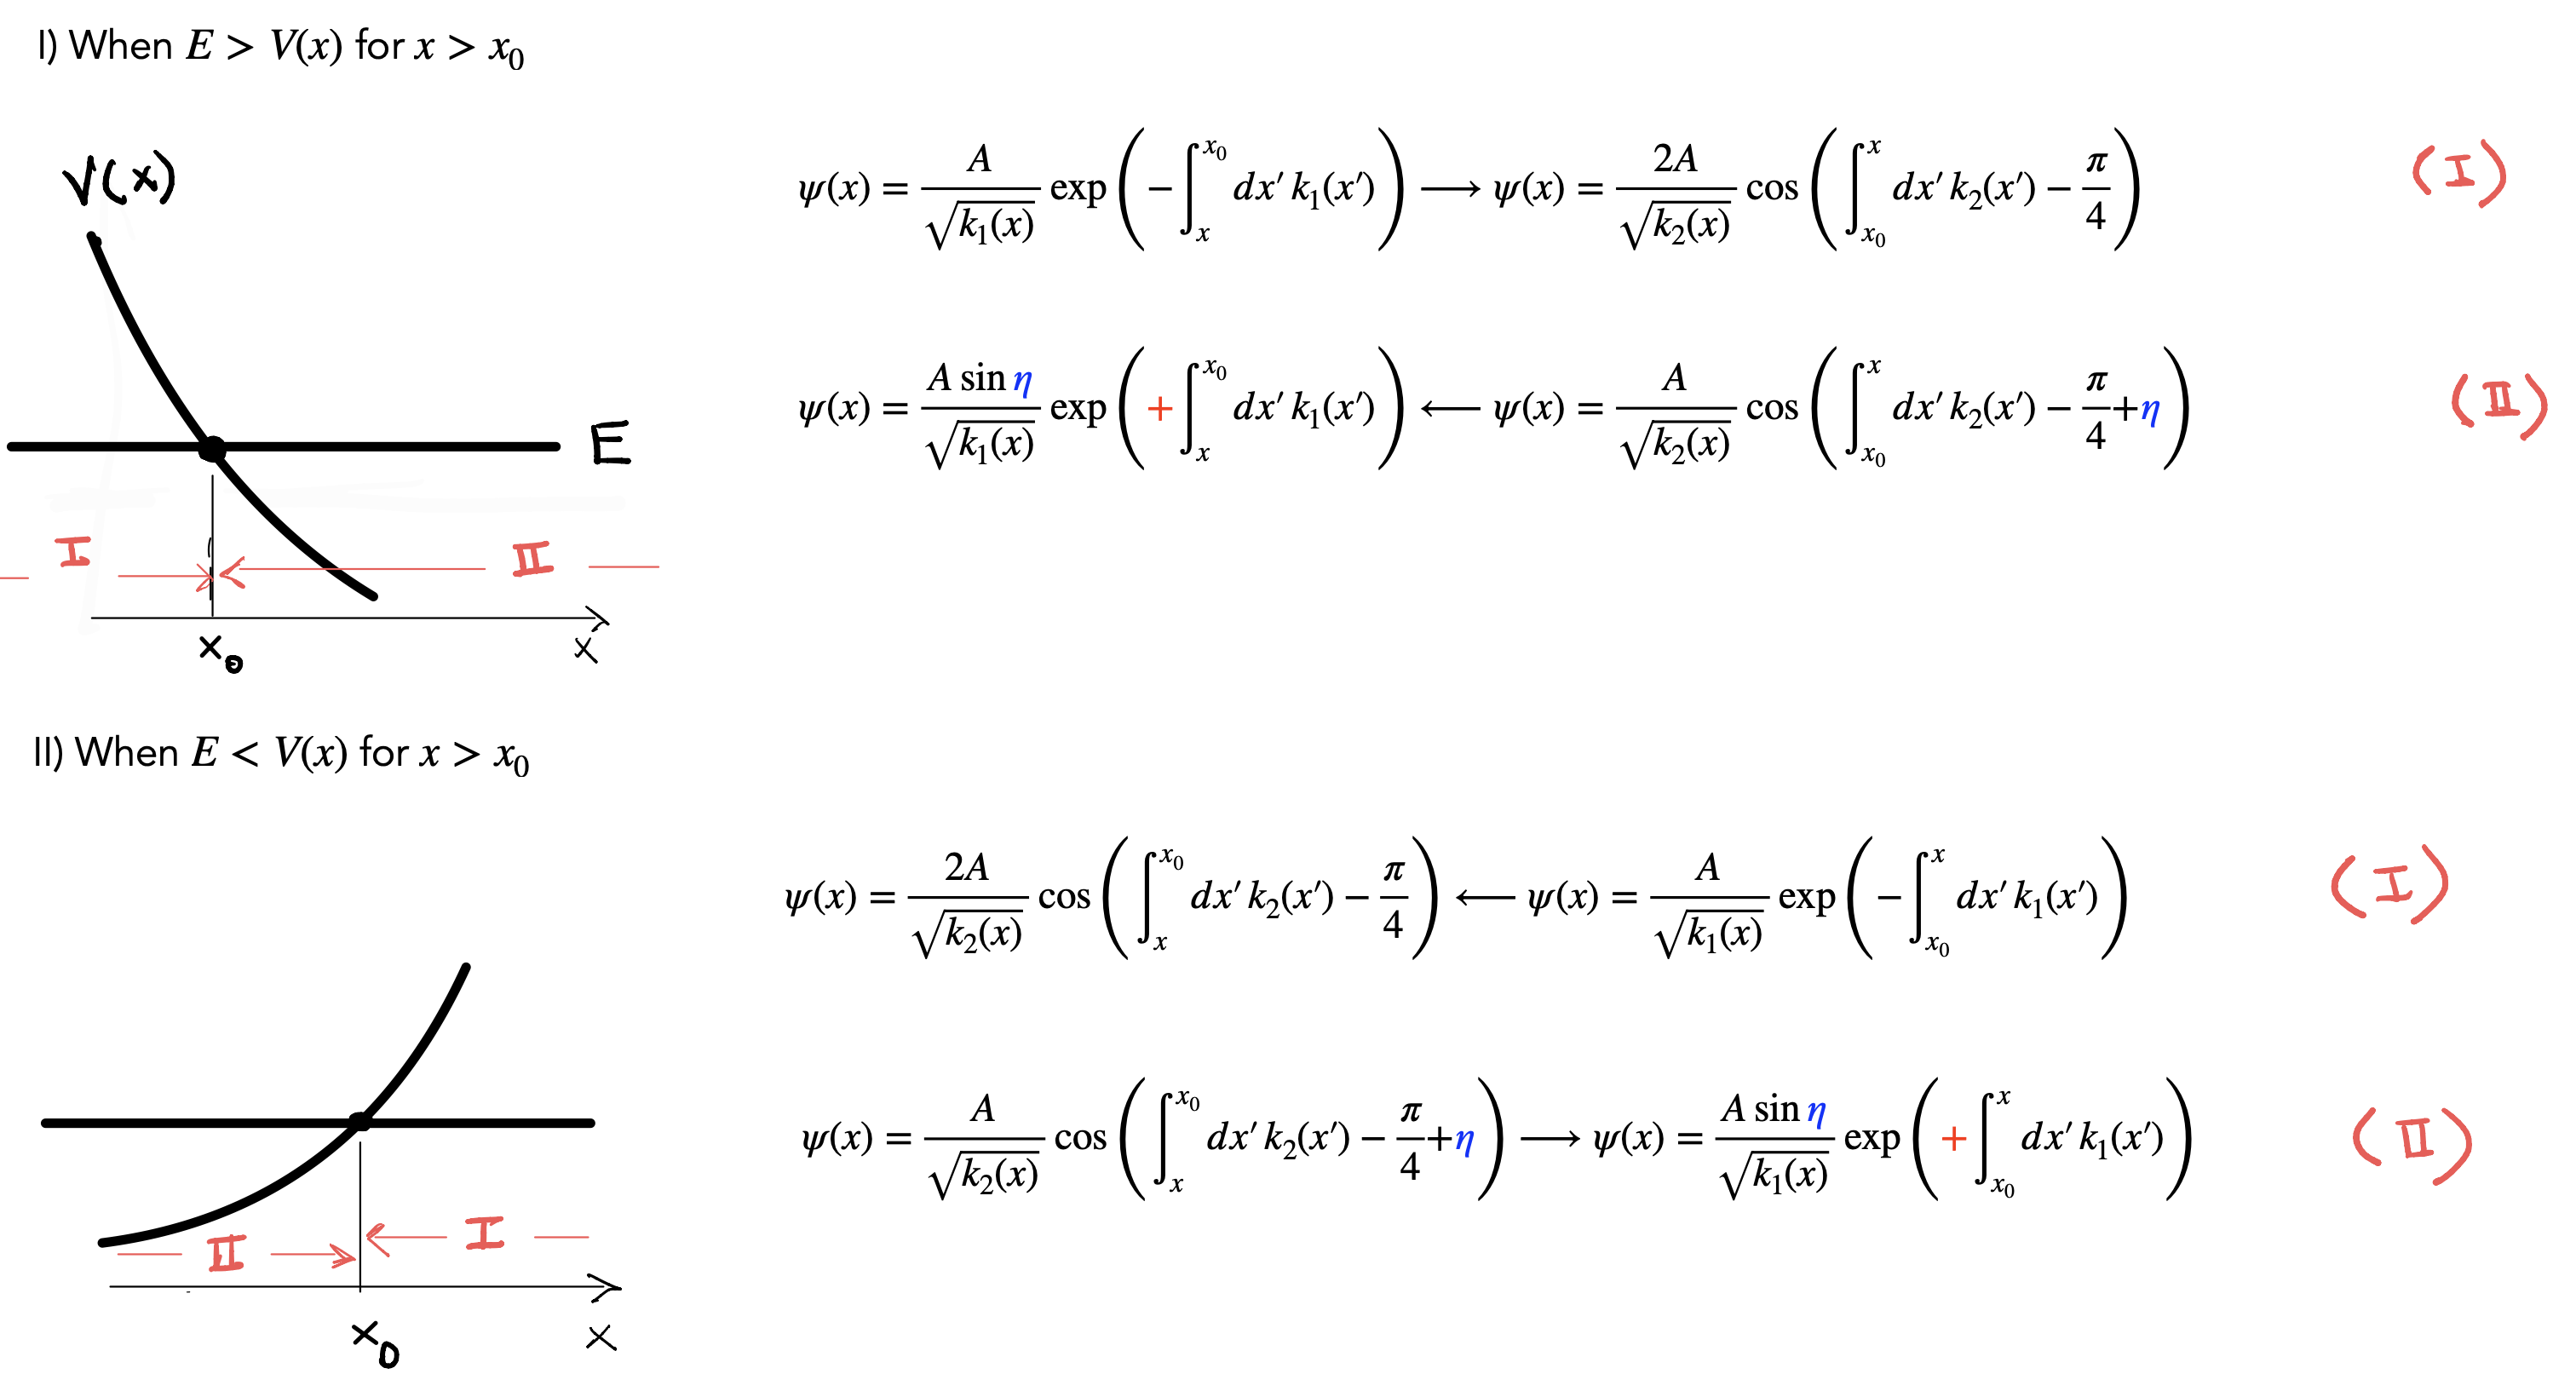
\includegraphics[width=1\linewidth]{src/WKB connection.png}
\end{figure}\end{center}

\subsection{Tunneling}
Consider scattering across rectangular barrier at $[0, L]$ with surrounding $V=0$. 
\[
    \psi(x) = \begin{cases}
        A\exp(ikx) + B\exp(-ikx) & x<0 \\ 
        \displaystyle 
        \df C {\sqrt{|p(x)|}}\exp\left(\df 1 \hb \int_0^x |p(x')|\, dx'\right) + 
        \df D {\sqrt{|p(x)|}}\exp\left(-\df 1 \hb \int_0^x |p(x')|\, dx'\right) & 0<x<L \\ 
        F\exp(ikx) & L<x
\end{cases}\] 
For large barriers, $C$ must be small so the The tunneling probability related 
by the decrease of the exponential decay term across the barrier. 
\begin{mdframed}
    \begin{equation}
        \label{eqn:wkb_tunneling}
        T = \left|\df F A\right|^2 \sim \exp\left(-\df 2 \hb \int_0^L |p(x)|\, dx\right)
    \end{equation}
\end{mdframed}
For general left-incident tunneling with regions $1, 2, 3$ 
being classically allowed, forbidden, and allowed, respectively. 
We have 
\malign{
    \psi_{1}(x) &= A\psi_{\mrm{WKB}, \rightarrow}(x) + B\psi_{\mrm{WKB}, \leftarrow}(x) \\ 
    \psi_{2}(x) &= C\psi_{\mrm{WKB}, \rightarrow}(x) + D\psi_{\mrm{WKB}, \leftarrow}(x) \\ 
    \psi_{3}(x) &= F\psi_{\mrm{WKB}, \rightarrow}(x)\\ 
}
This tunneling formula turns out to be useful not only for barriers with $0$ 
surrounding potentials but also general barriers. 
Using the connection formulas from $3\to 2\to 1$ relates 
$A, B$ as functions of $F$. The transmission coefficient coincides 
with equation~\ref{eqn:wkb_tunneling}. 
However, the reflection coefficient calculates to $R=|B/A|^2=1$. 
This violates the conservation of probability! 
We can only trust equation~\ref{eqn:wkb_tunneling} for $T\ll 1$. 

\subsection{Bound approximations}
The WKB approximation gives us an approximate wavefunction. 
Connection formulas give how approximations change across turning points 
at which a raw approximation would break down. 
Every confining potential possibly yields bound states. 
A consistent, normalizable connection of 3 approximations across 
classical turning points in the regions 
\begin{itemize}
    \item to the left of the confining potential (w.r.t. energy)
    \item inside the confining potential
    \item to the right of the confiniing potential 
\end{itemize}
yields the quantization condition for bound state energy. 

\subsubsection{Two infinite walls}
When there are two infinite vertical walls $x_-, x_+$ 
\begin{mdframed}
\[ 
    \int_{x_-}^{x_+}dx \, \sqrt{2m(E - V(x))} = \pi \hb n, \quad n=1, 2, \cdots 
\] 
\end{mdframed}
We begin by examining first case with two infinite vertical walls. 
Use the WKB approximation~\ref{eqn:wkb_wavefunction} with lower bound at $x_-$, then 
\[ 
    \psi_{\mrm{WKB}}(x_+) = \df 1 {\sqrt{p(x_+)}}
    \left(\alpha_1 \sin \phi(x_+) + \alpha_2\cos\phi(x_+)\right)=0, \quad 
    \phi(x) = \df 1 \hb \int_{x_-}^x p(x')\, dx' 
\] 
We have $\alpha_2=0$ by boundary condition at $x_-$. 
The equation above then yields the desired quantization condition $\phi(x_+) = 0$. 
\begin{example}[finite square well]
    Consider a finite square well with $V(x) -V_0$ in $[0, L]$ and zero elsewhere. 
    Applying the first approximation yields 
    \[ 
        \int_0^L dx\, \sqrt{2m(E + V_0)} = L\sqrt{2m(E + V_0)} = \pi n \hb 
        \implies E = \df{n^2\pi^2\hb^2}{2mL^2} - V_0
    \] 
    This is equivalent to a vertical shift of the infinite square well solution. 
    While there is no single quantitative metric for how good the approximation is 
    (as opposed to energy ratio), we can estimate by the magnitude of the next term in 
    the expansion. 
\end{example}

\subsubsection{One infinite wall}
When there is one infinite vertical wall at $x_-$, a smooth classical turning point at $x_+$
\begin{mdframed}
    \[ 
        \int_{x_-}^{x_+}dx\, \sqrt{2m(E - V(x))} = \pi \hb \left(n + \df 3 4\right), 
        \quad n = 0, 1, 2, \cdots 
    \] 
\end{mdframed}
Begin with an asymptotic formula for the decay on the right side of the potential. 
\[ 
    \psi_{x>x_+}(x) = \df{A}{\sqrt{k_1(x)}}\exp \left(-\df 1 \hb \int_{x_+}^x dx'\, k_1(x')\right)
\] 
Invoke connection at $x_+$ 
\[ 
    \psi_{x_-<x<x_+}(x) 
    = \frac{2A}{\sqrt{k_2(x)}} \cos \left(\df 1 \hb \int_{x}^{x_+} dx' k_2(x') - \frac{\pi}{4\hb } \right)
\] 
The boundary condition that $\psi_{x_-<x<x_+}(x_-)=0$ yields 
\[ 
    \int_{x}^{x_+} dx' k_2(x') = \pi \hb \left(n + \df 3 4\right)
\] 
\subsubsection{Two smooth turning points}
In case of smooth potential with classical turning points at $x_-<x_+$
\begin{mdframed}
    \[ 
        \int_{x_-}^{x_+} dx\, \sqrt{2m(E - V(x))} = \pi \hb \left(n + \df 1 2\right)
        ,\quad n = 0, 1, 2, \cdots 
    \]  
\end{mdframed}
Begin with an asymptotic formula for the decay on the right side of the potential 
\[ 
    \psi_{x>x_+}(x) = \df{A}{\sqrt{k_1(x)}}\exp \left(-\df 1 \hb \int_{x_+}^x dx'\, k_1(x')\right)
\] 
Invoke connection at $x_+$ and manipulate it to fit the connection formula at $x_-$. 
Here we temporarily omit $1/\hb$ to reduce clutter. 
\malign{
    \psi_{x_-<x<x_+}(x) 
    &= \frac{2A}{\sqrt{k_2(x)}} \cos \left( \int_{x}^{x_+} dx' k_2(x') - \frac{\pi}{4} \right) \\ 
    &= \frac{2A}{\sqrt{k_2(x)}} \cos \left( \left(\int_{x_-}^{x_+} - \int_{x_-}^{x}\right)
        dx' k_2(x') - \frac{\pi}{4} \right) \\ 
    &= \frac{2A}{\sqrt{k_2(x)}} \cos \left( \int_{x_-}^{x}dx'\, k_2(x') - \left(\int_{x_-}^{x_+}
        dx' k_2(x') + \frac{\pi}{4}\right)\right) \\ 
    &= \frac{2A}{\sqrt{k_2(x)}} \cos \left( \int_{x_-}^{x}dx'\, k_2(x') - \df \pi 4 - 
        \left(\int_{x_-}^{x_+}dx' k_2(x') - \frac{\pi}{2}\right)\right) \\ 
}
Invoke the connection formula at $x_-$ again with 
\[ 
    \eta =  \frac{\pi}{2\hb} - \df 1 \hb \int_{x_-}^{x_+}dx' k_2(x') 
\] 
In this classically forbidden region, $\psi_{x<x_-}(x)$ must be a decaying function yet 
the connection yields an increasing exponential. This yields the desired quantization 
condition $\sin\eta = 0$,  
\[ 
    \int_{x_-}^{x_+}dx' k_2(x') - \frac{\pi}{2} = n\pi \hb, \quad\quad n=0, 1, 2\cdots
\] 
The other quantization formulas follows from a similar procedure, with infinite vertical 
walls yielding zero boundary condition. 

% \subsection{Tunneling approximations}
% \begin{definition}[tunneling (transmission) coefficient]
%     A plane wave $\exp(-i(2mE) x)$ 
%     with kinetic energy $E$ incident upon a potential barrier in $[0, L]$ scatters with 
%     \malign{
%         \psi(x\leq 0) &= A\exp(ikx) + B\exp(-ikx)  \\ 
%         \psi(x\geq L) &= F\exp(ikx)
%     }
%     The transmission ratio is definined as 
%     \[ 
%         T = \df{|F|^2}{|A|^2}
%     \] 
%     The transmission ratio is defined generally in terms of the 
%     probability current $|J_{x>L}/J_{x<0}|$
% \end{definition}
% The WKB tunning coefficient is only appropriate in the low limit. 
% \leqalign{eqn:wkb_tunneling}{
%     T_{\mrm{WKB}}= \exp\left[-2\int_{x_-}^{x_+} dx\, \sqrt{2m(V(x) - E)}\right]\ll 1
% }

% To compute the tunneling coefficient, we start from the known expression for a 
% single transmitting plane wave traveling to the right from the barrier (which may 
% still be subject to the potential). 
% \malign{
%     \psi_{x>L}(x) 
%     &= \df{A}{\sqrt{k_2(x)}}\exp \left[i\int_L^x dx'\, k_2(x')\right] \\ 
%     &= \df{A}{\sqrt{k_2(x)}}\cos\left[i\int_L^x dx'\, k_2(x')\right] +
%         \df{Ai}{\sqrt{k_2(x)}}\cos\left[i\int_L^x dx'\, k_2(x') - \df \pi 2\right] \\ 
% }
% Recalling the connection formula, let $\eta = \pm \pi / 4$ for the first and second terms, 
% respectively. 
% \malign{
%     \psi_{0<x<L}(x) 
%     &= \df{A \sin (\pi / 4)}{\sqrt{k_1(x)}}\exp\left[\int_x^L dx'\, k_1(x')\right] +
%     \df{Ai\sin(-\pi / 4)}{\sqrt{k_1(x)}}\exp\left[\int_x^L dx'\, k_1(x')\right] \\ 
%     &= \df A {\sqrt{k_1(x)}} \exp\left[-i \df \pi 4 + \int_x^L dx'\, k_1(x')\right] \\ 
%     &= \df A {\sqrt{k_1(x)}} \exp\left[-i \df \pi 4 + \left(\int_0^L - \int_0^x \right)dx'\, k_1(x')\right] \\ 
% }
% Absorb the second integral into the coefficient and apply the connection formula again. 
% \[ 
%     \cdots 
% \] 
% Additionally, the reflection coefficient is $1$, violating $R+T=0$. 
% Therefore equation~\ref{eqn:wkb_tunneling} can only be trusted for $T_{\mrm{WKB}}\ll 1$. 